%\documentclass[envcountsect]{beamer}
\documentclass[envcountsect]{beamer}
%--------THEMES-------------------------------------------------
\usetheme{Boadilla}
%\usetheme{CambridgeUS}
%\usetheme{Dresden}
\usecolortheme{dolphin}
%\usetheme{Singapore}
\usefonttheme{default}
\usecolortheme{whale}
%---------------------------------------------------------------
%--------COLORS-------------------------------------------------
\setbeamercolor{frametitle}{fg=blue,bg=structure.fg!10!bg!50!bg}
\setbeamercolor{block title}{fg=blue,bg=structure.fg!10!bg!50!bg}
%---------------------------------------------------------------
%--------PACKAGES-----------------------------------------------
\usepackage{amsmath, amsthm, amssymb,amsfonts} 
\usepackage{graphicx,mathrsfs,fancyhdr,tabularx,listings,hyperref,color,picture,tikz,caption,subcaption}
\usepackage{wrapfig}
%\usepackage{enumitem}
%\usepackage[shortlabels]{enumitem}
\iffalse
\setbeamertemplate{itemize/enumerate body begin}
{\renewcommand\theenumii{\theenumi.\arabic{enumii}}}
\setbeamertemplate{enumerate subitem}{\theenumi.\arabic{enumii}} 
\fi
%################################
\AtBeginEnvironment{proof}{\footnotesize}
%\usepackage{graphicx,mathrsfs,amsfonts,tabularx,listings,picture,tikz,}
\usetikzlibrary{shapes,shadows,arrows,positioning,fit}
\definecolor{darkgreen}{rgb}{0.12,0.72,0.04}
\definecolor{darkred}{rgb}{0.76,0.16,0.08}
\definecolor{darkblue}{rgb}{0.22,0.07,0.75}

%-------FORMAT----------------------------------------------------------------------
%-----------------SHORT CUT----------------------------------------------------------

\newcommand{\bN}{\mathbb{N}}  \newcommand{\cN}{\mathcal{N}}
\newcommand{\bR}{\mathbb{R}}
\newcommand{\bC}{\mathbb{C}}
\newcommand{\bQ}{\mathbb{Q}}
\newcommand{\bE}{\mathbb{E}}
\newcommand{\bP}{\mathbb{P}}
\newcommand{\bT}{\mathbb{T}}
\newcommand{\F}{\mathcal{F}}
\newcommand{\M}{\mathcal{M}}
\newcommand{\A}{\mathcal{A}} 
\newcommand{\K}{\mathcal{K}}
\newcommand{\I}{\mathcal{I}}
\newcommand{\fF}{\mathbf{F}}

\newcommand{\remend}{}
\newcommand{\point}{\:\cdot\:}
\theoremstyle{definition}
\newtheorem{df}{Definition}[section]
\newtheorem*{rem}{Remark}
%\newcommand{\remend}{\hfill\text{$\diamond$}}
\setbeamertemplate{theorems}[numbered] % important!
\theoremstyle{plain}
\newtheorem{thm}[df]{Theorem}
\newtheorem{lem}[df]{Lemma}
\newtheorem{cor}[df]{Corollary}
\newtheorem{prop}[df]{Proposition}
%\setbeamertemplate{Lemmas}[numbered]
%\newcommand{\FRA}{\text{FRA}}
%\newcommand{\OIS}{\text{OIS}}
\definecolor{darkgreen}{rgb}{0.12,0.72,0.04}
\definecolor{darkred}{rgb}{0.76,0.16,0.08}
\definecolor{darkblue}{rgb}{0.22,0.07,0.75}

\newcommand*{\trans}[1]{#1^\mathfrak{t}} %matrix transpose
\newcommand*{\derivat}[4]{\frac{\partial #1_{#2}(#3)}{\partial #4}}
\newcommand*{\Deltabar}{\bar{\Delta}}
\newcommand*{\geninv}[1]{#1^{\leftarrow}}
\newcommand*{\udist}{\mathcal{U}(0,1)}
\newcommand*{\eqdist}{\overset{D}{=}}
%---------------------------------------------------------------
%-------THEOREM-------------------------------------------------
%\theoremstyle{definition}
%\newtheorem{df}{Definition}[section]
%\newtheorem*{rem}{Remark}
%\theoremstyle{plain}
%\newtheorem{thm}[df]{Theorem}
%\newtheorem{lem}[df]{Lemma}
%\newtheorem{cor}[df]{Corollary}
%\newtheorem{prop}[df]{Proposition}
%\newtheorem{ex}[df]{Example}
\setbeamertemplate{itemize items}[default]
%-----------OTHERS----------------------------------------------
\hypersetup{colorlinks=true, linkcolor=blue}

%---------------------------------------------------------------
\tikzstyle{decision} = [diamond,draw,fill=green!50]
\tikzstyle{line} = [draw,-latex']
\tikzstyle{elli} = [draw,align=center,rectangle,fill = green!20,minimum width=2cm, minimum height=1.2cm]
\tikzstyle{format} = [draw, thin, fill=green!]
\tikzstyle{medium} = [ellipse, draw, thin, fill=green!20, minimum height=2.5em]

%-----------TITLE SLIDE-----------------------------------------

%\vspace{2.5cm}
\title[\textcolor{white}{FRED-Talk}]{\textbf{\Large Copula Made Easy}}	
\subtitle{Session 1: Preliminaries}
%---------------------------------------------------------------
\author[T.~Nguyen]{\small{\bf Theanh~Nguyen}}
%---------------------------------------------------------------

\date[\tiny{Frankfurt a.~M., 2024}]{\small Frankfurt am Main, March~2024}
%\includegraphics[scale=0.01]{pics/tu-kl-logo.png}
%---------------------------------------------------------------
\begin{document}
\begin{frame}
\titlepage
\end{frame}
%--------------------------------------------
\begin{frame}
\frametitle{Agenda}
\tableofcontents
\end{frame}
%--------------------------------------------
\section{Preliminary Knowledge}
\begin{frame}
\tableofcontents[currentsection]
\end{frame}
\begin{frame}{Generalized Inverse (1/3)}
	\begin{df}[Generalized Inverse]
		Let $T: \bR \rightarrow \bR $ be an increasing function. Its {\it generalized inverse} is defined as 
		\begin{equation}
			\geninv{T}(y) := \inf\{x: T(x) \ge y\}.
		\end{equation}
	\end{df}

%\begin{wrapfigure}{l}{.5\textwidth}
\begin{figure}[]
	\label{fig:geninv}
	\centering
	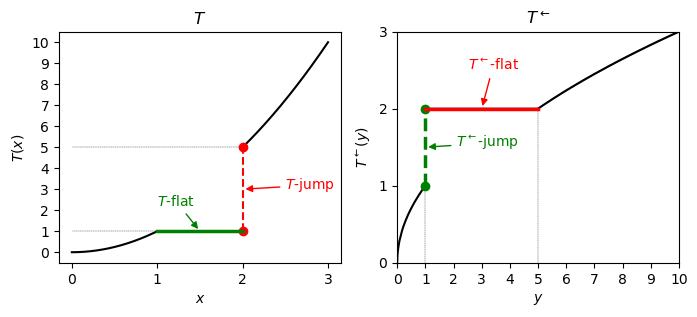
\includegraphics[scale=0.45]{figs/gen_inv.png}
\end{figure}
%\end{wrapfigure}
\begin{rem}
{\it Flat} parts of $T$ precisely correspond to {\it jumps} in $\geninv{T}$ and the jumps of $T$ precisely correspond to flat parts of  $\geninv{T}$.	
\end{rem}
\end{frame}
%====
\begin{frame}{Generalized Inverse (2/3)}
\begin{lem}[Basic properties of generalized inverse function] \label{geninv-lem}
	Let $T:\bR \rightarrow \bR$ be an increasing function. Then the following hold:
	\begin{enumerate}
		\item \label{geninv1} $\geninv{T}$ is an increasing, left continuous function with right limits (c\'agl\'ad or LCRL).
		\item \label{geninv2}$T$ is strictly increasing $\iff$ $\geninv{T}$ is continuous.
		\item  \label{geninv5} If $T$ is right continuous then $T(x) \ge y$ $\iff$ $x \ge \geninv{T}(y).$
		\item \label{geninv3} $T$ is strictly increasing  $\implies \geninv{T}(T(x)) = x$.
		\item \label{geninv4} $T$ is continuous $\implies$ $T(\geninv{T}(y)) = y$.
	\end{enumerate}
\end{lem}
\begin{proof}[Proof~(1/2)]
	For \ref{geninv1}: Note that for any $y_2 \ge y_1$, one has $\{x: T(x)\ge y_2\} \subseteq \{x: T(x)\ge y_1\}$ which implies $\geninv{T}(y_2)= \inf \{x: T(x)\ge y_2\}  \ge \inf \{x: T(x)\ge y_1\} = \geninv{T}(y_1)$. Hence, $\geninv{T}$ is increasing. This implies that $\{\geninv{T}(y-\epsilon)\}_{\epsilon>0}$ ($\{\geninv{T}(y+\epsilon)\}_{\epsilon>0}$) is increasing (decreasing) when $\epsilon \downarrow 0$ ($\epsilon \uparrow 0$) and bounded from above (below) by $\geninv{T}(y)$. 
\end{proof}
\end{frame}
%-------------
\begin{frame}{Generalized Inverse (3/3)}
	\begin{proof}[Proof~(2/2)]
		Thus, left (right) limit, $\geninv{T}(y-)$ ($\geninv{T}(y+)$), exists at any $y$ such that $\geninv{T}(y)<\infty$ ($\geninv{T}(y)>-\infty$).
		For the left-continuity of $\geninv{T}$ assume that there exists such $y$ with $\geninv{T}(y-) < \geninv{T}(y)$. Set $\delta:= \frac{\geninv{T}(y)-\geninv{T}(y-)}{2}>0.$ It follows from the definition of $\geninv{T}$ and the fact that $\geninv{T}(y-\epsilon) \le \geninv{T}(y-),\ \forall \epsilon >0$  that
		\begin{equation*}
			y-\epsilon \le T(\geninv{T}(y-\epsilon) + \delta) 
			\le T(\geninv{T}(y-) + \delta) =  T(\geninv{T}(y) - \delta) < y, \ \forall \epsilon >0. 
		\end{equation*}
	 	Letting $\epsilon \downarrow 0$ yields $y \le T(\geninv{T}(y) - \delta) < y$, a contradiction.\\
	 
		For \ref{geninv2}: See the plots in the first slide for a visual proof.
		
		For \ref{geninv5}: "$\implies$" is obvious. For "$\impliedby$", note that $T(\geninv{T}(y)) + \epsilon) \ge y \ \forall \epsilon >0$ (by the definition of infimum). Letting $\epsilon \downarrow 0$ and using right-continuity of $T$ yield $T(\geninv{T}(y)) =\lim_{\epsilon \downarrow 0} T(\geninv{T}(y)+\epsilon) \ge y$. Since $x \ge \geninv{T}(y)$ and $T$ is increasing, this implies that $T(x) \ge T(\geninv{T}(y)) \ge y$.
		
		For \ref{geninv3}: Note that $\geninv{T}(T(x)) \le x$. Assume $x > \geninv{T}(T(x))$. Set $\epsilon: = \frac{x-\geninv{T}(T(x))}{2} >0$. It follows then: $T(x) \le T(\geninv{T}(T(x)) + \epsilon ) = T(x-\epsilon)$, which is a contradiction as $T$ is strictly increasing. \\
		
		For \ref{geninv4}: Observe that for any $\epsilon>0$ one has $ T(\geninv{T}(y)  - \epsilon)<y \le T(\geninv{T}(y)  + \epsilon)$. Since $T$ is continuous, letting $\epsilon \downarrow 0$ yields $T(\geninv{T}(y)) = y$.
	
	\end{proof}
\end{frame}
%============
%-------------
\begin{frame}{Probability Integral Transform}
\begin{thm}[PIT - Probability Integral Transform]
\label{thm:pit}
Let $X$ be a random variable (rv) with cumulative distribution function (cdf) $F$ and $U$ be a standard uniform rv. Then the following hold:
	\begin{enumerate}
		\item $\geninv{F}(U) \eqdist X$, i.e. $\geninv{F}(U)$ has the same distribution as $X$.
		\item Moreover, if $F$ is continuous then $	F(X) \sim \udist$.
	\end{enumerate}
\end{thm}
\begin{proof}
	\begin{wrapfigure}{r}{3.5cm}
		\centering
		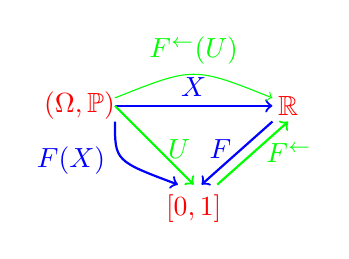
\begin{tikzpicture}
			\draw[blue,thick, ->] (0, 3) -- (2,3) ;
			\draw[blue,thick, ->] (2.0,2.8) -- (1.1,2);
			\draw[green, thick, ->] (1.3, 2) -- (2.2, 2.8);
			\draw[green, thick, ->] (0,3) -- (1.,2.0) ;
			\draw[green,->] (0,3.1) .. controls (1.0, 3.5).. (2.0,3.1);
			\draw[thick, blue, ->] (0, 2.8) .. controls (0,2.3) .. (0.8,2.0);
			\draw[red](-0.45,3)node{$(\Omega, \bP)$};
			\draw[red] (2.2, 3)node{$\bR$};
			\draw[red] (1.0,2.0)node[below]{$[0,1]$};
			\draw[green] (0.55, 2.45)node[right]{$U$};
			\draw[blue] (1.6, 2.45)node[left]{$F$};
			\draw[green] (1.8, 2.4)node[right]{$\geninv{F}$};
			\draw[green] (1.0, 3.4)node[above]{$\geninv{F}(U)$};
			\draw[blue] (1,3.0)node[above]{$X$};
			\draw[blue] (0,2.3)node[left]{$F(X)$};
		\end{tikzpicture}
	\end{wrapfigure}
	As $F$ is right-continuous, it follows from Lemma~\ref{geninv-lem}(\ref{geninv5}) that \[\{w\in \Omega: \geninv{F}(U(\omega)) \le x\} = \{\omega: U(\omega) \le F(x)\}.\] Hence, $\bP(\geninv{F}(U) \le x) = \bP(U\le F(x)) = F(x)$, i.e. $\geninv{F}(U)\sim X$.\\
	For the second statement, one has
	\[\bP(F(X) \le u) = \bP(X \le \geninv{F}(u)) = F(\geninv{F}(u)) = u.\] The last equality follows from Lemma~\ref{geninv-lem}(\ref{geninv4}), as $F$ is assumed to be continuous.
\end{proof}
\end{frame}
%----------
\begin{frame}{An Application of PIT- CCR Backtesting}
PIT plays a crucial role in copula theory. It also has many applications in statistics, e.g. for simulation (also called inverse transform sampling), distributional testing etc. Below is an application of PIT in backtesting of risk models.
	\begin{block}{Principle underlying the CCR Backtesting - PIT Approach}
		If a simulation model based on a distribution/ SDE were true, then \[ F_{model}(observation) \sim \udist.\]
	\end{block}
PIT approach is a popular CCR BT used by IMM banks:
\begin{itemize}
	\item For each set of simulated values (of a risk factor or portfolio) $S_1,...,S_N$, construct an empirical CDF.
	\item Convert the respective realization $S_0$ and all simulated scenarios $S_i$ via this CDF to obtain PIT values in $[0,1]$.
	\item Repeat the above for different initialization dates (e.g. multiple non-overlapping simulation periods). Determine a test statistics measuring "distance" between sim.~dist and uniform dist.
\end{itemize}
\end{frame}
\section{Copula}
\begin{frame}
	\tableofcontents[currentsection]
\end{frame}
\begin{frame}{Definition and Sklar's Theorem}
Given a joint CDF, one can easily obtain marginal distribution, e.g. via $P(X_1 \le x) = \bP(X_1\le x, X_2 < \infty)$. Conversely, given margins can one construct a joint CDF? Well... we need a dependence structure...

	\begin{block}{(Formal) Definition of Copula}
		A copula $C: [0,1]^d \rightarrow [0,1]$ is the CDF of a multivariate rv $U=(U_1,...,U_d)$ where $U_i \sim \udist,\ i=1,...,d$.
	\end{block}
\begin{thm}[Sklar]
	Let $F$ be a multivariate CDF with continuous margins $F_1,...,F_d$. Then there exists a unique copula $C: [0,1]^d \rightarrow [0,1]$ such that
	\begin{equation} \label{eq:sklar}
		F(x_1,..., x_d) = C(F_1(x_1),..., F_d(x_d)).
	\end{equation}
	Conversely, given a copula $C$ and univariate CDFs $F_1,..., F_d$ the function $F$ defined by \eqref{eq:sklar} is a joint CDF with margins $F_1,..., F_d$.
\end{thm}
\end{frame}
%###########
\begin{frame}{Auxiliary Results (1/2)}
To prove Sklar's theorem (and other copula-related results) we need the following:
	\begin{lem}\label{lem:geninv2}
		\begin{enumerate}
			\item \label{aux1} Let $X: (\Omega, \bP) \rightarrow \bR$ be a rv and $T: \bR \rightarrow \bR$ be an increasing function. Then
			\begin{equation} \label{eq:aux1}
				\bP(T(X)\le T(x)) = \bP(X\le x) + \bP(X>x, T(X)=T(x)).
			\end{equation}
			\item \label{aux2} If $F$ is a CDF, then
			\begin{equation} \label{eq:aux2}
				\bP(F(X)\le F(x)) = \bP(X\le x).
			\end{equation}
			\item  \label{aux3} Let $X=(X_1,...,X_d)$ be a multivariate rv with margins $\{F_i\}_{i=1}^d$. Then
			\begin{equation} \label{eq:aux3}
				\bP(F_1(X_1) \le F_1(x_1),..., F_d(X_d)\le F_d(x_d)) = \bP(X_1\le x_1,..., X_d\le x_d).
			\end{equation}
		\end{enumerate}
	\end{lem}
\end{frame}
\begin{frame}{Auxiliary Results (2/2)}
	\begin{proof}
		Note that as $\{X\le x\} \subseteq \{T(X)\le T(x)\}$, one has
		\begin{align*}
			\{T(X)\le T(x)\} &= \{X\le x\} \cup \left( \{T(X)\le T(x)\} \cap \{X > x\}\right) \\
			& = \{X\le x\} \cup \left( \{T(X)= T(x)\} \cap \{X > x\}\right), 
		\end{align*}
		where the second equality is due to $\{X >x \} \implies T(X) \ge T(x)$ (as $T$ is increasing). Eq.~\eqref{eq:aux1} follows then as the two sets above are disjoint.
		\eqref{eq:aux2} is implied directly from \eqref{eq:aux1}, where the second term vanishes in case $F$ is a CDF. Indeed, set $\gamma_x: = \sup \{z: z>x, F(z) = F(x)\}$: If $F(\gamma_x) = F(x)$, then
		$\bP(X>x, F(X) = F(x)) \le \bP(X\in (x, \gamma_x]) = F(\gamma_x) - F(x)=0$. 
		Otherwise, $\bP(X>x, F(X) = F(x)) \le \bP(X\in (x, \gamma_x)) = \lim_{n\to \infty}F(\gamma_x - 1/n) - F(x)=0$.\\
		Eq.~\eqref{eq:aux3} follows by noting that (using the same reasoning as used for \eqref{eq:aux2})
		\begin{equation*}
			\bigcap_{i=1}^d \{F_i(X_i) \le F_i(x_i)\} = \left(\bigcap_{i=1}^d \{X_i \le x_i\} \right) \bigcup E,
		\end{equation*} 
		where
		$ \left(\bigcap_{i=1}^d \{X_i \le x_i\} \right) \bigcap E = \emptyset$ and $\bP(E) = 0$.
	\end{proof}
\end{frame}
\begin{frame}{Sklar's Theorem - Proof}
	\begin{proof} [Proof of Sklar's Theorem]
		By Lemma~\ref{lem:geninv2}(\ref{aux3}), 
		\begin{equation} \label{eq:sklar1}
		\bP(F_1(X_1)\le F_1(x_1),..., F_d(X_d)\le F_d(x_d))  = \bP(X_1\le x_1, ..., X_d\le x_d) = F(x_1,...,x_d).
		\end{equation}
		Moreover, since $F_1,..., F_d$ are continuous $U_i:=F_i(X_i) \sim \udist,\ i=1,...,d$ by Theorem~\ref{thm:pit}. It follows that 
		\begin{equation}
			C(F_1(x_1),..., F_d(x_d)) = F(x_1,...,x_d)
		\end{equation}
		where $C$ is the copula specified as the CDF of $U=(U_1,...,U_d)$. For any $u=(u_1,...,u_d)\in [0,1]^d$, then due to Lemma~\ref{geninv-lem}(\ref{geninv4}):
		\begin{equation} \label{eq:sklar2}
			C(u_1,...,u_d) = C(F_1(\geninv{F_1}(u_1)),...,F_d(\geninv{F_d}(u_d)))
			= F(\geninv{F_1}(u_1),...,\geninv{F_d}(u_d)).
		\end{equation}
		Hence, $C$ is unique as represented by \eqref{eq:sklar2}.
		For the converse part, set $X_i:= \geninv{F_i}(U_i)$. By Theorem~\ref{thm:pit}, $X_i \sim F_i$. Moreover, by Lemma~\ref{geninv-lem}(\ref{geninv5}) and using \eqref{eq:sklar}:
		\begin{align}
			\bP(X_1\le x_1, ..., X_d \le x_d) &= \bP(U_1 \le F_1(x_1),..., U_d\le F_d(x_d)) = C(F_1(x_1),..., F_d(x_d)) \\
			& = F(x_1,...,x_d).
		\end{align}
	That means, $F$ is the joint CDF of $X = (\geninv{F_1}(U_1),..., \geninv{F_d}(U_d))$.
	\end{proof}
\end{frame}
%===============
\begin{frame}{Sklar's Theorem: Important Remarks}
Formulae \eqref{eq:sklar} and \eqref{eq:sklar2} are fundamental in working with copulae:
\begin{itemize}
	\item Eq.~\eqref{eq:sklar} implies that {\tt Joint Distribution = Copula + Margins}, it shows how a joint distribution $F$ is formed by coupling together margins via copula $C$.
	\item Eq.~\eqref{eq:sklar2} $C(u_1,...,u_d) = F(\geninv{F_1}(u_1),...,\geninv{F_d}(u_d))$ shows how a copula is extracted from a multivariate distribution with continuous margins. It shows how copulae express dependence on a quantile scale: $C(u_1,...,u_d)$ is the joint probability of $\{X_i
	 \le u_i - \text{quantile}\}$.
\end{itemize}
Sklar's theorem also allows us to define copula for a continuous joint distribution/ multivariate rv with continuous margins:
\begin{df}[Copula of a continuous random vector/distribution]
	If the multivariate rv $X$ has joint CDF $F$ with continuous marginal distributions $F_1,..., F_d$, the the copula of $X$ (or $F$) is the CDF $C$ of $(F_1(X_1),..., F_d(X_d))$.
\end{df}
\end{frame}
%===============
\begin{frame}{Invariance Principle}
	\begin{thm}[Invariance via strict monotonic transformation]
		Let $X=(X_1,...,X_d)$ be a multivariate random variable with continuous margins $F_1,..., F_d$. Let $C$ be the copula of $X$ and $T_1,..., T_d$ be strictly increasing functions.  Then 
		\[Y = (Y_1, ..., Y_d) := (T_1(X_1), ..., T_d(X_d))\]
		has the same copula as $X$.
	\end{thm}
\begin{proof}
	Denote by $G, G_1,..., G_d$ and $F, F_1, ...,F_d$ joint- and marginal CDFs of $X$ and $Y$, respectively. We first prove that
	$G_i = F_i \circ \geninv{T_i}, \ i = 1,...,d.$
	Indeed, 
	\begin{align}
		\label{eq:inva-temp} \nonumber
		F_i \circ \geninv{T_i}(y) = \bP(X_i \le \geninv{T_i}(y)) &=  \bP(\geninv{T_i}(T_i(X_i))\le \geninv{T_i}(y))\\ 
		& = \bP(T_i(X_i) \le y) + \bP(T_i(X_i) > y, X_i = \geninv{T_i}(y)),
	\end{align} 

\end{proof}
\end{frame}
%===============
\begin{frame}{Invariance Principle (Cont.)}
	\begin{proof}[Proof (cont.)]
		where \eqref{eq:inva-temp} follows from Lemma~\ref{geninv-lem}(\ref{geninv3}) and Lemma~\ref{lem:geninv2}(\ref{aux1}). The second term in the last equality of \eqref{eq:inva-temp} is zero as $F_i$ is continuous, leading to:
		\begin{equation*}
			F_i \circ \geninv{T_i}(y) = \bP(X_i \le \geninv{T_i}(y)) = \bP(T_i(X_i) \le y) = G_i(y),\ \text{i.e. } G_i = F_i \circ \geninv{T_i}.
		\end{equation*}
		Hence, $G_i\circ T_i = F_i \circ \geninv{T_i} \circ T_i = F_i$ due to Lemma~\ref{geninv-lem}(\ref{geninv3}). 
		Thus,
		\begin{align}
			\label{eq:inva-temp1}
			C(u_1,..., u_d) & = \bP(F_1(X_1) \le u_1,..., F_d(X_d) \le u_d )\\ 
			& = \bP(G_1\circ T_1(X_1) \le u_1,..., G_d\circ T_d(X_d) \le u_d )\\
			& = \bP(G_1(Y_1) \le u_1,..., G_d(Y_d) \le u_d).
		\end{align}
	Hence, $Y=(Y_1,...,Y_d)$ has copula $C$ as $G_1,...,G_d$ are continuous since $\geninv{T_1},...,\geninv{T_d}$ are continuous due to Lemma~\ref{geninv-lem}(\ref{geninv2}). Note that \eqref{eq:inva-temp1} follows as $C$ is the copula of $X$.
	\end{proof}
\end{frame}
%==============
%===============
\begin{frame}{Many more in the next sessions (upon continued interest)}
	\begin{itemize}
		\item What does the invariance principle mean in finance?
		\item Fr\'echet bounds and fundamental copula.
		\item Copula simulation.
		\item Explicit (Archimedian) and implicit (via continuous distributions) copulae.
		\item Correlations and copula.
		\item Copula and tail dependence.
		\item Applications in risk management.
		\item Deep learning copula.
		\item This list is not exhaustive.
	\end{itemize}
\end{frame}

\iffalse
\begin{frame}{What does monotone invariance mean in Finance?}
	Inhalt...
\end{frame}
\begin{frame}{Copula bounds}
\begin{lem}[Fr\'echet bounds]
	Copula has the following bounds:
	\begin{equation} \label{eq:frechet_bound}
		\max \left(0, \sum_{i=1}^{d} u_i + 1 -d \right) \le C(u_1,...,u_d) \le \min(u_1,...,u_d).
	\end{equation}
\end{lem}
\begin{proof}
		Note that $C(u_1,...,u_d) = \bP( \bigcap_{i=1}^{d} \{U_i \le u_i\})$ and 
		$\bigcap_{i=1}^{d} \{U_i \le u_i \} \subseteq \{U_i \le u_i \}$, for $i=1,...,d.$
		Hence, $C(u_1,..., u_d) \le \min_{i=1,...,d} \bP(U_i \le u_i) = \min(u_1,..., u_d).$
		For the lower bound, re-write the joint CDF as follows:
		$C(u_1,..., u_d) = 1- \bP\left( \bigcup_{i=1}^{d} \{U_i > u_i\}\right)$
		and note that
		$\bP\left( \bigcup_{i=1}^{d} \{U_i > u_i\}\right) \le \sum_{i=1}^{d} \bP( U_i > u_i) = d - \sum_{i=1}^{d} u_i.$
		This combined with the fact that $C(u)\ge 0$ yields:
		\[ \max\left(0, \sum_{i=1}^{d} u_i + 1 -d\right) \le C(u_1,...,u_d). \]
\end{proof}
\end{frame}
%========
\begin{frame}{Fundamental Copulae}
1. Fundamental Copula:

\end{frame}
\fi
%-------THANK YOU----------------------------
\begin{frame}
\begin{center}
\Large{\textcolor{blue}{\bf Thank you for your attention!}}\\

\Large{ \textcolor{blue}{\bf Questions?} }
\end{center}
\end{frame}
%--------------------------------------------
%\begin{frame}{References}
%	\begin{thebibliography}{}
%		
%		\bibitem[Constantinides (1992)]{Constantinides} Constantinides,~G.~M.~(1992): A theory of the nominal term structure of interest rates, \textit{Review of Financial Studies} {\bf 5} (4), 531-552.
%		\bibitem[Flesaker \& Hughston (1996)]{FH96} Flesaker,~B. \& L.~P.~Hughston~(1996): Positive interest, \textit{Risk} {\bf 9}, 46-49.
%		
%		\bibitem[Goldberg (1998)]{Goldberg98} Goldberg, L.~R.~(1998): Volatility of the short rate in the rational lognormal model, {\it Finance and Stochastics} {\bf 2} (2), 199-211.
%		
%		\bibitem[Jin/Glasserman~(2001)]{Jin-Glasserman} Jin,~Y. \& P.~Glasserman~(2001): Equilibrium positive interest rates: A unified view, {\it Review of Financial Studies}, {\bf 14} (1), 187-214.
%		\bibitem[Rogers (1997)]{Rogers1997} Rogers,~L.~C.~G.~(1997): The potential approach to the term structure of interest rates and foreign exchange rates, \textit{Mathematical Finance} {\bf 7} (2), 157-164.
%		
%		\bibitem[Rutkowski (1997)]{Rutkowski1997} Rutkowski, M.~(1997): A note on the Flesaker-Hughston model of the term structure of interest rates, \textit{Applied Mathematical Finance} {\bf 4} (3), 151-163. 
%		
%		\bibitem[Yao (2001)]{Yao01} Yao, Y.~(2001): State price density, Esscher transforms, and pricing options on stocks, bonds, and foreign exchange rates, {\it North American Actuarial Journal} {\bf 5} (3), 104-117.
%	\end{thebibliography}
%\end{frame}
\end{document}
